\documentclass[spanish, c]{beamer}

\usepackage[utf8]{inputenc}
\usepackage[spanish, mexico]{babel}
\usepackage{amsmath}
\usepackage{mathtools}
\usepackage{hyperref}
\usepackage{xcolor}
\usepackage{color}
\usepackage{ragged2e}
\usepackage{mathrsfs}
\usepackage{csquotes}
\usepackage{listings}
\usepackage[scaled]{beramono}
\usepackage[T1]{fontenc}
\usepackage{matlab-prettifier}
\usepackage{graphicx}
\usepackage{booktabs}
\usepackage{tikz}
\usepackage{venndiagram}
\usepackage{semantic}

\renewcommand{\indent}{\hspace*{2em}}

% \usetikzlibrary{fit, shapes, arrows}

% \usepackage{courier}
% \usepackage{subfigure}
% \usepackage{enumerate}
% \usepackage{algorithmic}
% \usepackage{algorithm}

% \usepackage{listings}
% \usepackage{lstlinebgrd}

\usetheme{Boadilla}
\usefonttheme[onlymath]{serif}

\newcommand{\matlab}[1]{\lstinline[style=Matlab-editor]!#1!}
\newcommand\blfootnote[1]{%
\begingroup
\renewcommand\thefootnote{}\footnote{#1}%
\addtocounter{footnote}{-1}%
\endgroup
}

\lstset
{
    language = Matlab,
    style = Matlab-editor,
    basicstyle = \mlttfamily\scriptsize,
    escapechar = `,
    numbers = left,
    frame = tb,
}

\lstdefinestyle{output}
{
    language = {},
    basicstyle = \mlttfamily\scriptsize,
    escapechar = `,
    numbers = none,
    showtabs = false,
   	showstringspaces = false,
}

% Sets the templates
\definecolor{navyblue}{RGB}{0, 0, 128}
\definecolor{crimson}{RGB}{128, 16, 0}

\setbeamertemplate{navigation symbols}{}
\setbeamertemplate{headline}{}
\setbeamertemplate{title page}[default][colsep=-4bp,rounded=true]
\setbeamertemplate{footline}[frame number]
\setbeamertemplate{bibliography item}[text]
\setbeamertemplate{theorems}[numbered]

\setbeamercolor{title}{fg=navyblue, bg=white}
\setbeamercolor{frametitle}{fg=navyblue, bg=white}
\setbeamercolor{structure}{fg=navyblue}
\setbeamercolor{button}{fg=white,bg=navyblue}

\setbeamercovered{transparent}

\title{Teoría de Grafos}
\subtitle{Matemáticas Discretas \\ (TC1003)}
\author{
    \texorpdfstring{
        \begin{center}
            M.C. Xavier Sánchez Díaz \\
            \href{mailto:sax@tec.mx}{\texttt{sax@tec.mx}}
        \end{center}
    }
    {M.C. Xavier Sánchez Díaz}
}

\institute[Tecnológico de Monterrey]{\includegraphics[scale=0.5]{../img/logo}}
\date{}

\begin{document}

\setlength{\rightskip}{0pt}

\begin{frame}[plain]
    \titlepage        
\end{frame}

\begin{frame}{Outline}
    \tableofcontents
\end{frame}

\section{Introducción}

\begin{frame}{Teoría de Grafos}{Introducción}

    Un \alert{grafo} es una \textbf{estructura matemática} ordenada que, como otras estructuras de datos, son representaciones de algún objeto con características dadas. \pause

    \bigskip

    \begin{block}{Definición formal}
        Un grafo $G$ es una \textbf{tupla} $G = (V, E)$, donde $V$ es un \textbf{conjunto} de \alert{vértices} (o \textbf{nodos}) y $E$ es un conjunto de \alert{ejes} (o \textbf{conexiones}).
    \end{block} \pause

\end{frame}

\begin{frame}{Origen de la teoría de grafos}{Introducción}
    
    \begin{center}
        \Huge
        Story time:\\
        \textit{Los puentes de Konisberg}
    \end{center}

\end{frame}

\section{Aplicaciones I}

\begin{frame}{Redes Computacionales}{Aplicaciones}
    \begin{center}
        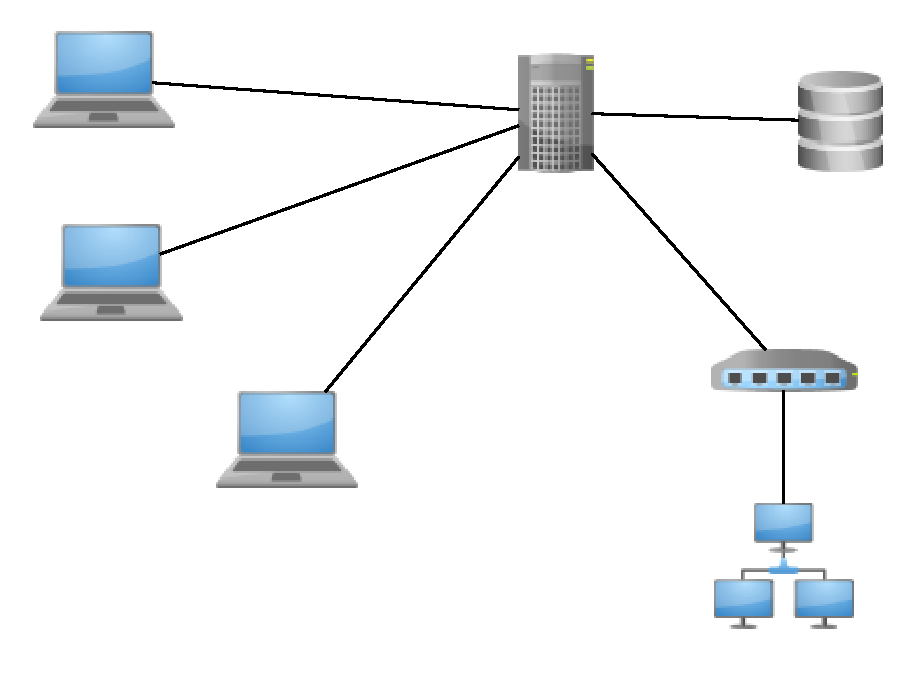
\includegraphics[width=0.6\textwidth]{network.pdf}
    \end{center}
\end{frame}

\begin{frame}{Redes Sociales}{Aplicaciones}
    \begin{center}
        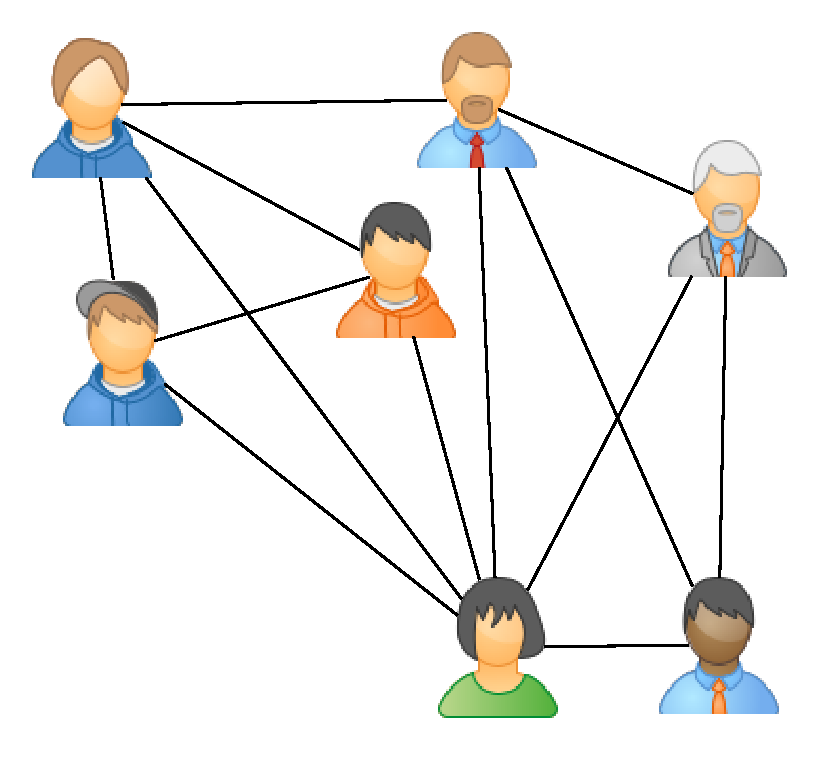
\includegraphics[width=0.6\textwidth]{social.pdf}
    \end{center}
\end{frame}

\begin{frame}{O sea, relaciones}{Aplicaciones}
    \begin{center}
        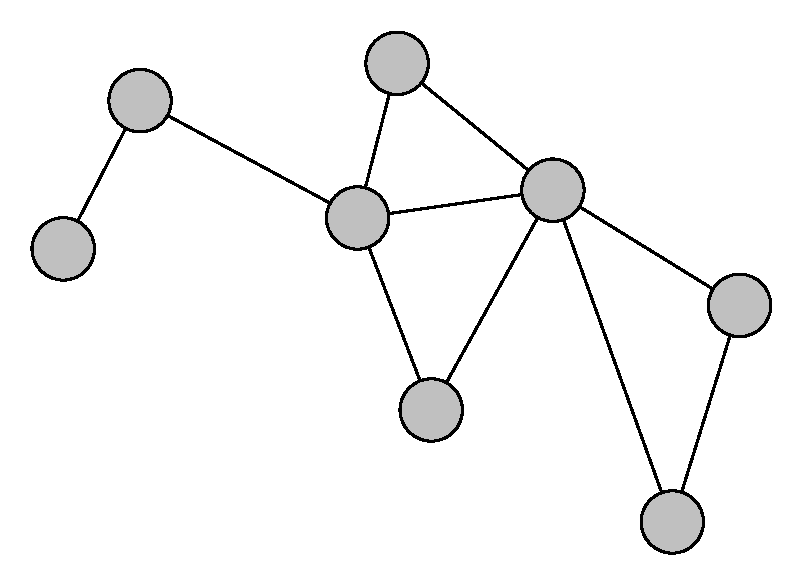
\includegraphics[width=0.4\textwidth]{graph01.pdf}
    \end{center}

    \begin{columns}
        \begin{column}{0.5\textwidth}
            \begin{itemize}
                \item Locaciones
                \item Personas
                \item Variables
            \end{itemize}
        \end{column}
        \begin{column}{0.5\textwidth}
            \begin{itemize}
                \item Números
                \item Estados
                \item Conjuntos
            \end{itemize}
        \end{column}
    \end{columns}
\end{frame}

\begin{frame}{Relaciones no necesariamente bidireccionales}{Aplicaciones}
    \begin{center}
        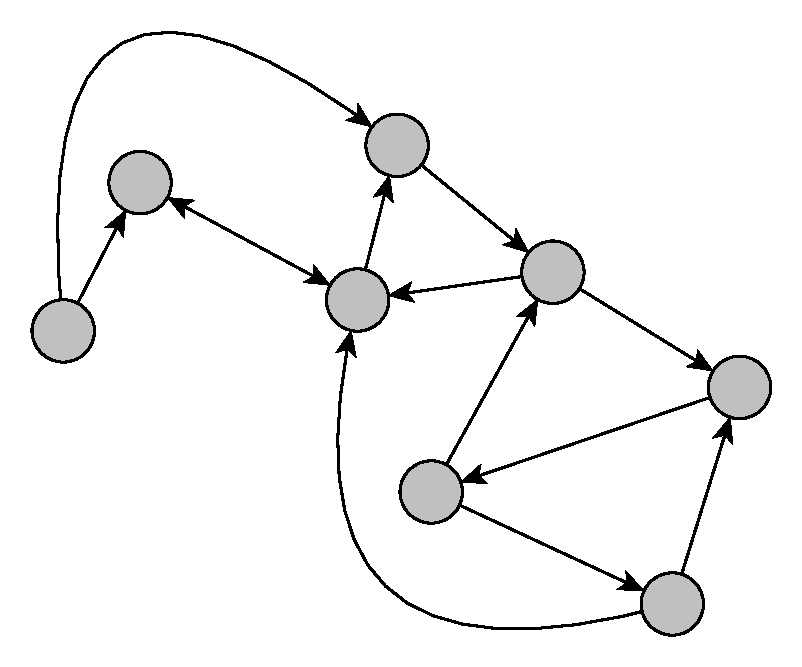
\includegraphics[width=0.5\textwidth]{digraph01.pdf}
    \end{center}

    \bigskip

    Cuando un \textbf{grafo} tiene ejes con dirección, se le conoce como \alert{grafo direccionado} o \textbf{digrafo}.
\end{frame}

\section{Vocabulario}

\begin{frame}{Vocabulario}
    \begin{center}
        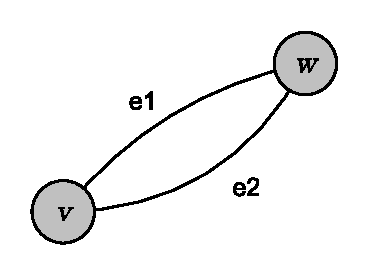
\includegraphics[width=0.3\textwidth]{extremes.pdf}
    \end{center}

    \begin{block}{Extremos y paralelos}
        \begin{itemize}
            \item Dos vértices $v$ y $w$ son \textbf{extremos} de los ejes $e_1$ y $e_2$
            \item Los ejes $e_1$ y $e_2$ son \textbf{paralelos} (porque conectan los mismos nodos)
        \end{itemize}
    \end{block}

    \bigskip

    Esto nos sugiere la idea de una función $f: V \to V$ para \textit{generar} el conjunto de \textbf{ejes} $E$.
\end{frame}

\begin{frame}{\textit{Oh god} más vocabulario}
\begin{itemize}[<+->]
    \item Un eje de la forma $(v, v)$ es un \textbf{ciclo}\blfootnote{\tiny Casi nada en \texttt{alert} y casi todo en \texttt{textbf} porque no espero se aprendan todo esto}
    \item Se dice que un grafo es \textbf{simple} si no tiene \textbf{ejes paralelos} o \textbf{ciclos}
    \item Un grafo en el que $E = \emptyset$ es un grafo \textbf{vacío}
    \item Un grafo en el que $E = V = \emptyset$ es un grafo \textbf{nulo}
    \item Un grafo en el que $\vert V \vert = 1$ es un grafo \textbf{trivial}
    \item Dos \textbf{ejes} son \alert{adyacentes} si \textbf{comparten} un \textbf{vértice}
    \item Dos \textbf{vértices} $u$ y $v$ son \alert{adyacentes} si existe un \textbf{eje} $(u,v)$ o $(v,u)$
    \item El \alert{grado} de un vértice $v$, $deg(v)$, es el número de ejes donde $v$ es un extremo (los ciclos cuentan doble)
    \item Un vértice $v$ es \textbf{pendiente} si $deg(v) = 1$
    \item Un vértice $v$ está \textbf{aislado} si $deg(v) = 0$
    \item El \alert{vecindario} de un vértice $v$ es el \textbf{conjunto de vértices adyacentes} de $v$
\end{itemize}
\end{frame}

\begin{frame}{\textit{Walks, Trails, Paths, Circuits, Components\dots}}{\textit{pls stop}}

    \begin{itemize}[<+->]
        \item Una \alert{caminata} (\textit{walk}) es una secuencia de nodos y ejes alternados: saliendo de un nodo \textbf{inicial} $v_{i_0}$ y llegando a un nodo \textbf{final} $v_{i_k}$
        \item Dos \textbf{vértices} están \alert{conectados} si existe una \alert{caminata} entre ellos
        \item Una \textbf{caminata} es \textbf{abierta} si $v_{i_0} \neq v_{i_k}$, o \textbf{cerrada} si $v_{i_0} = v_{i_k}$
        \item Un \textbf{sendero} (\textit{trail}) es una caminata en donde cada eje visitado se recorre una sola vez.
        \item Un \textbf{sendero} es un \textbf{camino} (\textit{path}) si cualquier vértice es visitado a una sola vez, a excepción del inicial y el final.
        \item Un \textbf{camino} cerrado es un \alert{circuito} (o ciclo\footnote{Total BS, yo sé. Lo siento; así es esto.})
        \item Un grafo es \alert{completo} si todos los vértices están conectados al resto. También se le conoce como \textbf{grafo conectado}
    \end{itemize}
\end{frame}

\begin{frame}{Lo siento, en serio}

    \begin{itemize}[<+->]
        \item Un grafo $G'=(V',E')$ es un \alert{subgrafo inducido} de $G = (V ,E)$ si $V' \subset V$ y si $E'$ es el conjunto de ejes que conectan a $V'$.
        \item Un subgrafo $G'$ es un \alert{componente} de $G$ si $G'$ es un \textbf{grafo conectado} y $G'$ es un \textbf{subgrafo inducido} por aquellos ejes de $G$ que tengan uno de sus extremos en $G'$.
        \item $\sum_i^n deg(v_i) = 2\vert E\vert$ (La suma de todos los grados de un grafo es el doble del número de ejes)
        \item $\sum_i^n deg(v_i) \mod 2 = 0$ (Por lo mismo, la suma de todos los grados de un grafo es un número par)
        \item $\lvert\{v : deg(v) \mod 2 = 1\}\rvert \mod 2 = 0$ (El número de vértices de un grafo que tienen grado impar, es un número par)
    \end{itemize}

\end{frame}

\begin{frame}    
    \begin{center}
        \LARGE
        Operaciones y problemas con grafos los vemos la próxima semana
    \end{center}
\end{frame}
% \section*{Referencias}

% \begin{frame}[t]{Referencias}
    % \nocite{bibID01}
    % \nocite{bibID02}

    % \bibliographystyle{IEEE}
    % \bibliography{biblio}
% \end{frame}

\end{document}